\documentclass{article}
\usepackage[margin=1in]{geometry}
\usepackage{amsmath,amsfonts,amssymb}
\usepackage{listings}
\usepackage{color}
\usepackage{graphicx}
\usepackage{subfig}
\usepackage{blkarray}
\usepackage{multirow}
\usepackage{float}
\usepackage{caption}
\usepackage{subcaption}
\begin{document}
\begin{titlepage}
	\setlength{\parindent}{0pt}
	\large

\vspace*{-2cm}

\definecolor{dkgreen}{rgb}{0,0.6,0}
\definecolor{gray}{rgb}{0.5,0.5,0.5}
\definecolor{mauve}{rgb}{0.58,0,0.82}

\lstset{frame=tb,
  language=Python,
  aboveskip=3mm,
  belowskip=3mm,
  showstringspaces=false,
  columns=flexible,
  basicstyle={\small\ttfamily},
  numbers=none,
  numberstyle=\tiny\color{gray},
  keywordstyle=\color{blue},
  commentstyle=\color{dkgreen},
  stringstyle=\color{mauve},
  breaklines=true,
  breakatwhitespace=true,
  tabsize=3
}

University of Waterloo \par
CS 480 \par
\vspace{0.05cm}
r2knowle: 2023-11-13
\vspace{0.2cm}

{\huge Exercise \# 3 \par}
\hrule

\vspace{0.5cm}
\textbf{Q3a)} For this question we are going to derive both the expectation step and the maximization step independently: \\\\
\textbf{Expectation Step: } To begin we are given that $S_k$ is diagonal, which gives us the following properties:
\[ |S_k| = \sigma_1^2 \times \sigma_2^2 \times ... \times \sigma_n^2 = \prod_i^n \sigma_i^2 \]
\[ S_k^{-1} = \begin{bmatrix}
\frac{1}{\sigma_1^2} & ... & 0 \\
\vdots & & \vdots \\
0 & & \frac{1}{\sigma_n^2} \\
\end{bmatrix} \]
Continuing from the slides the we get that:
\begin{align*}
r_{ik} &= q_i(Z_i = k) \\
&= p_{\theta}(Z_i = k | x_i) \\
&= \frac{ p_{\theta} (Z_i = j, x_i)} { p_{\theta}(x_i)} \\
&= \frac{ \pi_k N(\mu_k, S_k, x_i) } { \sum^k_{l=1} \pi_k N(\mu_l, S_l, x_i))}
\end{align*}
Note that the denominator is calculated outside of the red step, and the red step is only the numerator. Therefore any optimization for a diagonal matrix will have to occur within $p_{\theta} (Z_i = j, x_i)$, thus we get the following expansion:
\begin{align*}
\pi_k N(\mu_k, S_k, X_i) &= \frac{1}{\sqrt{ \lvert 2\pi S_k \rvert }} \text{exp}\left( - \frac{1}{2}(x_i - \mu_k)^T S_k^{-1}(x_i - \mu_k) \right) \\
&= \frac{1}{\sqrt{  2\pi^k  \lvert S_k \rvert }} \text{exp}\left( - \frac{1}{2} \left( \frac{(x_{i1}-\mu_{k1})^2}{\sigma_1^2} + \frac{(x_{i2}-\mu_{k2})^2}{\sigma_2^2} + ... + \frac{(x_{in}-\mu_{kn})^2}{\sigma_n^2}  \right) \right) \\
&= \frac{\text{exp}\left( - \frac{1}{2} \left( \frac{(x_{i1}-\mu_{k1})^2}{\sigma_1^2} + \frac{(x_{i2}-\mu_{k2})^2}{\sigma_2^2} + ... + \frac{(x_{in}-\mu_{kn})^2}{\sigma_n^2}  \right) \right)}{\sqrt{  2\pi^k  \sigma_1^2 \times \sigma_2^2 \times ... \times \sigma_n^2}} \\
&= \frac{\text{exp}\left( - \frac{1}{2} \frac{(x_{i1}-\mu_{k1})^2}{\sigma_1^2} \right)}{\sqrt{  2\pi  \sigma_1^2}} \times \frac{\text{exp}\left( - \frac{1}{2} \frac{(x_{i2}-\mu_{k2})^2}{\sigma_2^2} \right)}{\sqrt{  2\pi  \sigma_2^2}} \times ... \times \frac{\text{exp}\left( - \frac{1}{2} \frac{(x_{in}-\mu_{kn})^2}{\sigma_n^2} \right)}{\sqrt{  2\pi  \sigma_n^2}}\\
\end{align*}
\newpage
\textbf{Maximization Step}
As given in the slides are our is to maximize the following:
\[ p_\theta(x) = \sum^k_i \pi_k N(\mu_k, S_k, x_i) \]
Which from the slides can we know can be rewritten as:
\begin{align*}
&=  \text{argmax}_\theta \sum^n_{i=1}\sum_{j=1}^k q_i(Z_i = j) \log p_\theta(x_i, Z_i = j)  \\
&= \text{argmax}_\theta \sum^n_{i=1}\sum_{j=1}^k q_i(Z_i = j) \log \left[ \frac{\pi_k}{\sqrt{\lvert 2\pi S_k \rvert}}\text{exp}\left( - \frac{1}{2}(x_i - \mu_k)^T S_k^{-1}(x_i - \mu_k) \right) \right]\\
&= \text{argmax}_\theta \sum^n_{i=1}\sum_{j=1}^k q_i(Z_i = j) \left[ \log \left( \pi_k \right) - \frac{k}{2} \log \left( 2\pi \right) - \frac{1}{2}\log \left(\lvert S_k \rvert \right) + \left( - \frac{1}{2}(x_i - \mu_k)^T S_k^{-1}(x_i - \mu_k) \right) \right] \\
&= \text{argmax}_\theta \sum^n_{i=1}\sum_{j=1}^k r_{ik} \left[ \log \left( \pi_k \right) - \frac{k}{2} \log \left( 2\pi \right) - \frac{1}{2}\log \left(\lvert S_k \rvert \right) + \left( - \frac{1}{2}(x_i - \mu_k)^T S_k^{-1}(x_i - \mu_k) \right) \right] 
\end{align*}
We can then take the derivative w.r.t to $S_k$ and set to zero, to find where this is concave function is maximized:
\begin{align*}
\sum^n_{i=1}\sum_{j=1}^k r_{ik} \left[ \log \left( \pi_k \right)' - \frac{k}{2} \log \left( 2\pi \right)' - \frac{1}{2}\log \left(\lvert S_k \rvert \right)' + \left( - \frac{1}{2}(x_i - \mu_k)^T S_k^{-1}(x_i - \mu_k) \right)' \right]  &= 0 \\
\sum^n_{i=1}\sum_{j=1}^k r_{ik} \left[ 0 - 0 - \frac{1}{2}\log \left( \prod_i^n \sigma_i^2 \right)' + \left( - \frac{1}{2}(x_i - \mu_k)^T (x_i - \mu_k) \right) \right]  &= 0 \\
\sum^n_{i=1}\sum_{j=1}^k r_{ik} \left[ 0 - 0 - \frac{1}{\sigma_{ik}^2}  + \left( - \frac{1}{2}(x_i - \mu_k)^T (x_i - \mu_k) \right) \right]  &= 0 
\end{align*}
We can rearrange to get:
\begin{align*}
\sum^n_{i=1} \frac{ r_{ik}}{\sigma_{ik}^2} &= \sum^n_{i=1} \frac{1}{2}(x_i - \mu_k)^T (x_i - \mu_k) \\
S_k &= \sum^n_{i=1} \frac{ \frac{1}{2}(x_i - \mu_k)^T (x_i - \mu_k)}{r_{ik}}\\\\
\end{align*}
On the next page is my implementation of the algorithm.
\newpage
\begin{lstlisting}
import matplotlib.pyplot as plt
import numpy as np
import pandas as pd
from numpy.random import RandomState

TOL = 1e-5

def estep(x_i, mu, s, d):
    currentSum = 0
    for idx in range(0, d):
        step1 = (x_i[idx] - mu[idx]) ** 2 / s[idx] * -0.5
        step2 = np.log(np.sqrt(2 * np.pi * np.abs(s[idx])))
        currentSum += step1 - step2
    return currentSum

def mstep(x, r, elementSum, mu, cluster, d, N):
    step1 = 0
    for i in range(N):
        step1 += np.exp(r[i, cluster]) * x.iloc[i, d] ** 2

    step2 = step1 / elementSum[cluster]
    return step2 - mu[cluster, d] ** 2


def train(X, maxIter, k):
    N, D = X.shape

    pi = np.ones(k) / k
    mu = np.random.rand(k, D)

    r = np.zeros((N, k))
    s = np.ones((k, D))

    pastError = 0

    log_likelihood = 0

    for iter in range(maxIter):

        print("Start of E Step")
        # E step
        clusterSum = np.zeros(N)
        for i in range(N):
            for cluster in range(k):
                r[i, cluster] = np.log(pi[cluster])
                r[i, cluster] += estep(X.iloc[i], mu[cluster], s[cluster], D)

            for cluster in range(k):
                clusterSum[i] += np.exp(r[i, cluster])

            for cluster in range(k):
                r[i, cluster] -= np.log(clusterSum[i])

        # Error Check
        pastError = log_likelihood
        log_likelihood = 0
        for i in range(N):
            step3 = 0
            for cluster in range(k):
                step1 = X.iloc[i] - mu[cluster]
                step2 = np.exp(-0.5 * step1 @ np.linalg.inv(np.diag(s[cluster])) @ step1.T)
                step3 += step2 / np.sqrt(pi[cluster] * np.prod(s[cluster]))
            log_likelihood += np.log(step3)

        log_likelihood = log_likelihood * -1

        if iter > 1 and pastError - log_likelihood <= TOL * log_likelihood:
            break
        print("Current Error is: ", log_likelihood)
        # M Step
        elementSum = np.zeros(k)
        for cluster in range(k):
            for i in range(N):
                elementSum[cluster] += np.exp(r[i, cluster])

        for cluster in range(k):
            pi[cluster] = elementSum[cluster] / N

        for cluster in range(k):
            for d in range(D):
                localSum = 0
                for i in range(N):
                    localSum += (np.exp(r[i, cluster])) * X.iloc[i, d]
                mu[cluster, d] = localSum / elementSum[cluster]

        for cluster in range(k):
            for d in range(D):
                s[cluster, d] = mstep(X, r, elementSum, mu, cluster, d, N)

        print("Done M Step")
    return log_likelihood, pi, mu, r, s


gmm = pd.read_csv("gmm_dataset.csv", header=None)

yVals = []
xVals = []

last = 0
for i in range(1, 11):
    log_likelihood, pi, mu, r, s = train(gmm, 500, i)

    print(i)
    xVals.append(i)
    yVals.append(log_likelihood)
    last = log_likelihood


plt.plot(xVals, yVals)
plt.xlabel("Number of Gaussian Distributions (k)")
plt.ylabel("Negative Log Likelihood")
plt.title("")
plt.show()
\end{lstlisting}
\newpage
\textbf{Time and Space Complexity Analysis: } For the expectation step we need to loop through each cluster and element of x, as well as each feature which gives us a time complexity of O(NDK). For the loss function we need to only loop through clusters and N so we get a time complexity of O(ND). For the maximization step we need to loop through each element of x, each feature and each cluster so its only O(NDK) time. Therefore the total time complexity is:
\[ O(NDK) \]
As for space complexity we need to store the following variables:
\begin{align*}
pi &= O(K) \\
mu &= O(KD) \\
r &= O(NK) \\
s &= O(KD) \\
\end{align*}
\textbf{Graph and Analysis: } 
\begin{center}
 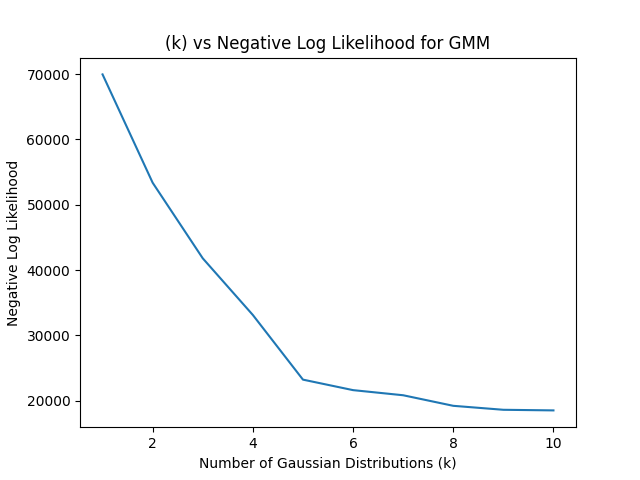
\includegraphics[width=.7\linewidth]{q3aplot.png} \\
 \end{center}
The best choice of k in this case is 5. As we can see in the graph that's where a hinge occurs so after that point the marginal benefit in log loss decreases (but is not negative). \textbf{The model parameters are provided in a seperate csvs.}
\newpage
\textbf{Q3b)} For this question we get the following graph, where for k = 5 we got a test error of roughly $22.17\%$ seen below is the graph:
\begin{center}
 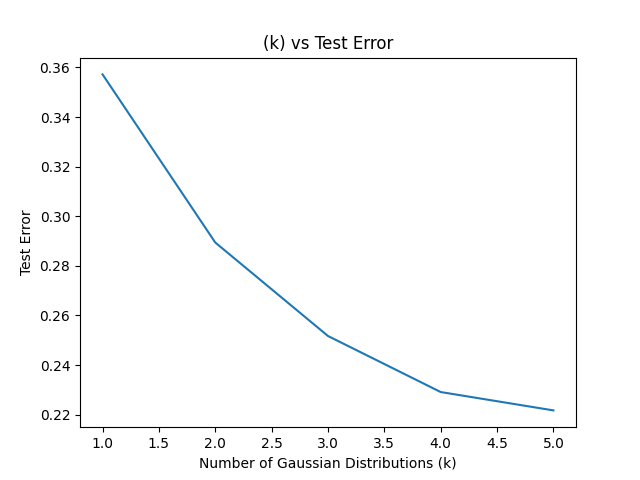
\includegraphics[width=.7\linewidth]{q3b.png} \\
 \end{center}
The code used to generate this graph is seen below, although repeated members arent included:
\begin{lstlisting}
import matplotlib.pyplot as plt
import numpy as np
import pandas as pd
import tensorflow as tf

from sklearn.decomposition import PCA

def normalize_img(image):
    scaled_image = image / 255.  # Scale the image to 0-1

    return scaled_image.flatten()


(x_train, y_train), (x_test, y_test) = tf.keras.datasets.mnist.load_data()


dataToTrain = []
dataToTest = []

for i in range(0, len(x_train)):
    dataToTrain.append(normalize_img(x_train[i, :]))

for i in range(0, len(x_test)):
    dataToTest.append(normalize_img(x_test[i, :]))

pca = PCA(n_components=100)
pca.fit(dataToTrain)

dataToTrain = pca.transform(dataToTrain)
dataToTest = pca.transform(dataToTest)

dataToTrainByDigit= [[] for i in range(10)]

for i in range(0, len(x_train)):
    dataToTrainByDigit[y_train[i]].append(dataToTrain[i,:])


predictionPerDigit = []
for i in range(0, 10):
    predictionPerDigit.append(len(dataToTrainByDigit[i])/len(x_train))


xVals = []
yVals = []
for k in range(1, 6):
    correct = 0
    incorrect = 0

    modelsPerDigit = []


    for i in range(0, 10):
        modelsPerDigit.append(trainGMM(k, dataToTrainByDigit[i]))


    for test_idx in range(0, len(dataToTest)):

        prob = calculatePredictions(modelsPerDigit[0], dataToTest[test_idx])
        digitWithHighestProb = 0

        for i in range(1, 10):

            likelihood = calculatePredictions(modelsPerDigit[i], dataToTest[test_idx])
            if prob < likelihood * predictionPerDigit[i]:
                prob = likelihood * predictionPerDigit[i]
                digitWithHighestProb = i

        if digitWithHighestProb == y_test[test_idx]:
            correct += 1
        else:
            incorrect += 1

    xVals.append(k)
    yVals.append(incorrect/ (correct+incorrect))
    print(k, ": ", incorrect/ (correct+incorrect))

plt.plot(xVals, yVals)
plt.xlabel("Number of Gaussian Distributions (k)")
plt.ylabel("Test Error")
plt.title("(k) vs Test Error")
plt.show()
\end{lstlisting}
\end{titlepage}
\end{document}